\chapter{Attachments}
\label{appendix:attachments}

This appendix summarizes the submitted electronic attachment package: the pruned source code snapshot used to build the prototype, the external build/dependency boundaries, and the hardware/calibration artifacts required to reproduce the physical setup.

\section{Submission package, source code, and third-party software}
\label{appendix:source_code}

\minihead{Development repository.}
The development history of the project is available at \url{https://github.com/medk42/diploma-thesis-code}.
The electronic attachment submitted with this thesis contains a pruned snapshot intended for building and inspection; it may not correspond to a single stable tagged revision of the development repository.
\xxx{Update this link if the maintained repository is moved/split. Optionally add a tag/commit hash if a stable release is created. --> keep this one}

\minihead{Top-level structure of the submitted attachment.}
The attachment package is organized as follows (paths are relative to the attachment root):

\begin{description}
  \item[\path{camera/}] Calibration artifacts (Charuco PDF, camera mount CAD).
  \item[\path{diploma-thesis-code/}] Pruned C++ source tree (core + helpers + modules).
  \item[\path{pen/}] Pen CAD + firmware.
  \item[\path{robot/aergo_interface_cbun/}] Robot-side component (CBun) source tree.
  \item[\path{scene/}] Example scene CAD model.
  \item[\path{third_party_licenses/}] License texts for vendored components.
  \item[\path{LICENSE}, \path{NOTICE}, \path{README.md}, \path{THIRD_PARTY_NOTICES.md}] Root metadata and notices.
\end{description}

\minihead{Included vs.\ excluded code scope.}
The submitted code snapshot includes:
\begin{itemize}
    \item the core runtime and module contract (\path{diploma-thesis-code/backend/core/}, \path{diploma-thesis-code/backend/module_common/}),
    \item the interface helpers and shared message formats (\path{diploma-thesis-code/backend/module_helpers/}),
    \item the concrete modules used by \autoref{fig:runtime_full} (\path{diploma-thesis-code/default_modules/}),
    \item build configuration and dependency manifests (\path{diploma-thesis-code/manifests/}, \path{diploma-thesis-code/vcpkg-triplets/}).
\end{itemize}

The submitted snapshot intentionally excludes development-only and non-essential repository content (e.g., demos and retired modules) and does not redistribute third-party binaries.

\minihead{Build quickstart (core runtime + modules).}
The project is implemented in C++ and uses CMake with presets together with vcpkg (manifest mode) to obtain third-party dependencies.
A typical build workflow is:

\minihead{Prerequisites.}
\begin{itemize}
    \item C++23-capable toolchain (Windows: MSVC; Linux: modern GCC/Clang).
    \item CMake and a multi-configuration Ninja generator (``Ninja Multi-Config'').
    \item vcpkg installed from its Git repository; environment variable \type{VCPKG\_ROOT} must point to the vcpkg repository root.
\end{itemize}

\minihead{Configure and build.}
From \path{diploma-thesis-code/}:

\begin{verbatim}
cmake --list-presets
cmake --preset core-windows
cmake --build --preset core-windows-Release
\end{verbatim}

Alternatively build Debug via \texttt{core-windows-Debug}. On Linux, use \texttt{core-linux} instead of \texttt{core-windows} and the corresponding build presets
(\texttt{core-linux-Release}, \texttt{core-linux-Debug}).

\minihead{Dependency build note.}
The first configuration will trigger vcpkg to download and compile the project’s external dependencies (including transitive dependencies).
This step can take a long time on a fresh machine (from tens of minutes up to several hours, depending on hardware and cache state).
Subsequent configurations/builds typically reuse cached artifacts.

\minihead{Install step (required runtime layout).}
After building, the install step assembles a self-contained runtime tree under \path{binaries/}
(core executable, module dynamic library binaries, and per-module data such as frontend \path{docroot/}).
Some tests and the runtime expect this installed layout.

\begin{verbatim}
cmake --install build-core-windows --config Release
\end{verbatim}

\minihead{Run.}
After installation:
\begin{verbatim}
cd binaries
.\core.exe modules data
\end{verbatim}
By default, the web frontend is available at \texttt{http://localhost:8080}.
The default port is configured by the frontend module via \path{diploma-thesis-code/default_modules/frontend_module/module_data/config.txt}
(and after installation via the corresponding runtime copy under \path{binaries/data/frontend_module/config.txt}).

\minihead{Third-party dependencies and licensing boundary.}
This thesis distributes the implementation as source code only (no third-party binaries).
Third-party software falls into two categories:

\begin{itemize}
    \item \textbf{External dependencies (not redistributed).}
    These are obtained separately (via vcpkg) and remain under their upstream licenses.
    The direct dependencies used by the core build are declared in \path{diploma-thesis-code/manifests/core/vcpkg.json} and pinned by the vcpkg \texttt{builtin-baseline} in that manifest.
    \item \textbf{Vendored components (redistributed in-tree).}
    A small number of files (web assets, fonts, and derived firmware/design files) are included directly in the attachment and remain under their original licenses.
    Their license texts are provided in \path{third_party_licenses/} and summarized in \path{THIRD_PARTY_NOTICES.md}.
\end{itemize}

\minihead{Project license.}
All original work in the submitted attachment is licensed under the Apache License 2.0 (see \path{LICENSE} and \path{NOTICE} at the attachment root).
Vendored components remain under their upstream licenses as described above.

\minihead{Note on \type{base64.hpp}.}
The project vendors a header-only Base64 implementation at
\path{diploma-thesis-code/backend/module_helpers/base_64/include/websocketpp/base64.hpp}.
Its original permissive notice is preserved in-file and also duplicated in \path{third_party_licenses/base64_notice.txt} for convenience.

\section{Hardware and calibration artifacts}
\label{appendix:artifacts}

\subsection{Charuco board (calibration target)}
\label{appendix:charuco}

The attachment includes an A4-ready Charuco calibration target exported via OpenCV:
\path{camera/charuco_pattern_A4.pdf}.
For printing, the intended usage is to print at 100\% scale and mount the sheet on a flat rigid backing.
The pattern was printed on standard A4 paper with default print settings; scaling was disabled, and the printed square size was measured to confirm it matches the intended dimensions.

The calibration module uses the following Charuco board parameters (compile-time defaults):
\begin{itemize}
    \item grid: $8 \times 12$ (rows $\times$ columns),
    \item square length: $0.024\,\mathrm{m}$, marker length: $0.018\,\mathrm{m}$,
    \item dictionary: \type{DICT\_4X4\_100},
    \item legacy pattern enabled.
\end{itemize}

These values are defined in \path{diploma-thesis-code/default_modules/robot_stereo_camera_calibration_module/include/calib/charuco_defaults.h}.

\subsection{Robot-mounted stereo camera mount (CAD)}
\label{appendix:camera_mount_cad}

The mechanical mount used to attach the stereo camera to the Kassow robot is provided as:
\path{camera/stereo_camera_robot_mount.step}.
This mount realizes the ``rigid robot-mounted stereo rig'' assumption discussed in \autoref{subsec:ch4_hw_robot}.

\subsection{Pen CAD and firmware}
\label{appendix:pen_artifacts}

The custom pen CAD model is provided as:
\path{pen/pen.step}.
The pen firmware is provided as:
\path{pen/pen_firmware.ino}.

The firmware is derived from the upstream D-Point project (Jcparkyn/dpoint) and modified for this thesis prototype; the upstream license text is included under \path{third_party_licenses/}.
The mechanical design is original work for this thesis prototype, with high-level inspiration taken from D-Point.

For reference, the internal layout is shown in \autoref{fig:app_pen_internals}.

\begin{figure}[h]
    \centering
    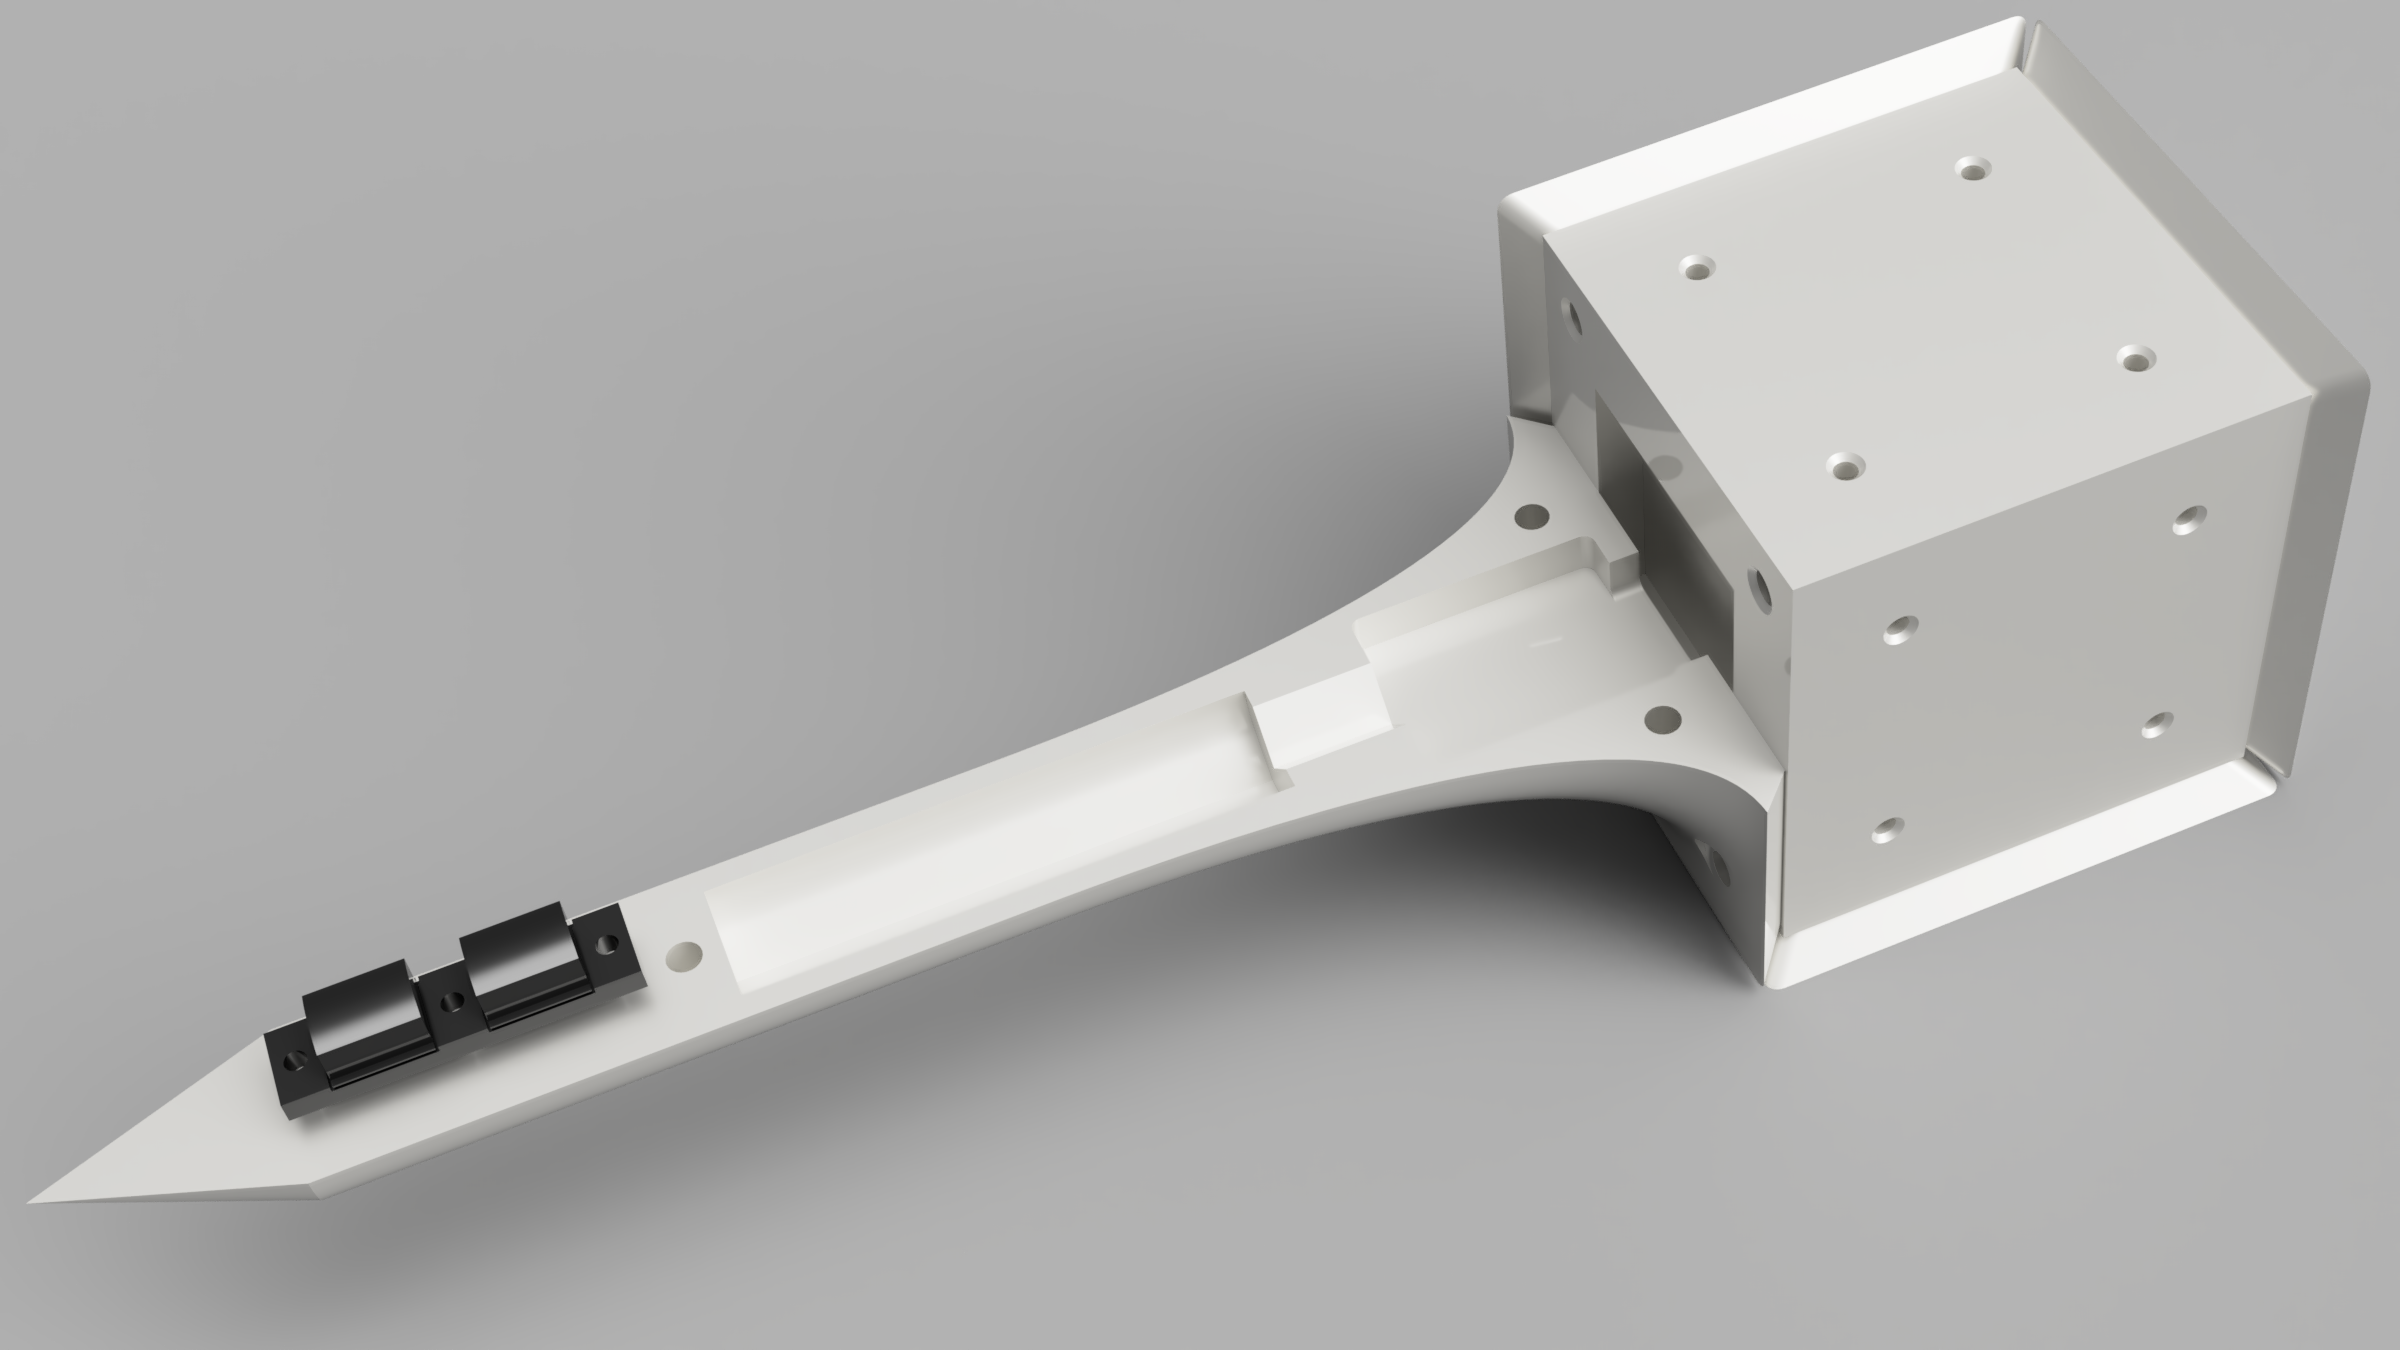
\includegraphics[width=0.92\linewidth]{img/appendix/pen_partial_internals_bg.png}
    \caption[Pen internal layout (CAD renders)]{Pen internal layout (CAD renders): a partial view highlighting the electronics compartment, the button assembly, and the cube to which the ArUco codes are attached.}
    \label{fig:app_pen_internals}
\end{figure}

\minihead{Pen assembly.}
The pen body is intended for FDM printing and screw assembly.
The electronics are based on a \type{Seeed Studio XIAO nRF52840 Sense} powered from a single-cell Li-ion battery (\type{INR10440} form factor).
Two momentary buttons provide the primary/secondary input; the firmware configures them as active-low inputs with internal pull-ups on pins \type{D1} (primary) and \type{D2} (secondary).
Use a small momentary switch variant that fits the CAD pocket and wire the buttons using thin flexible wire.

\minihead{Recommended screw lengths.}
Holes are sized for thread-forming into printed plastic.
\begin{itemize}
    \item Button plate: $3\times$ M1.5, length $3\,\mathrm{mm}$.
    \item Pen top to pen bottom: $1\times$ M3, $8$--$10\,\mathrm{mm}$; and $2\times$ M3, $14$--$16\,\mathrm{mm}$.
    \item Bottom tip to pen bottom: $2\times$ M3, $4$--$5\,\mathrm{mm}$.
    \item Pen to cube: $4\times$ M3, $8$--$10\,\mathrm{mm}$.
    \item Marker plates to cube: $5\times(4\times)$ screws (total 20), M2, $6$--$8\,\mathrm{mm}$.
\end{itemize}

\minihead{Practical assembly sequence.}
Wire the two buttons (to \type{D1}/\type{D2} and \type{GND}) and mount them in the handle; connect the battery to the MCU board and secure the battery and MCU in the housing (e.g., foam or adhesive for strain relief).

Flash \path{pen/pen_firmware.ino} and verify BLE advertising (\type{"3D Pen"}) and button reporting.
Close the pen body and attach the bottom tip. Finally, mount the five marker plates to the cube and attach the cube to the pen body.

\subsection{3D printing layout (informative)}
\label{appendix:printing_layout}

The pen components were manufactured using consumer FDM 3D printing. The print plate arrangement used for manufacturing the pen parts is shown in \autoref{fig:app_print_layout}. The parts were printed on a Bambu Lab P1S with AMS using default settings for generic PLA on the \type{0.20mm Standard} profile, with support-interface material enabled (white/black PLA and support PLA, switched via AMS).

\begin{figure}[h]
    \centering
    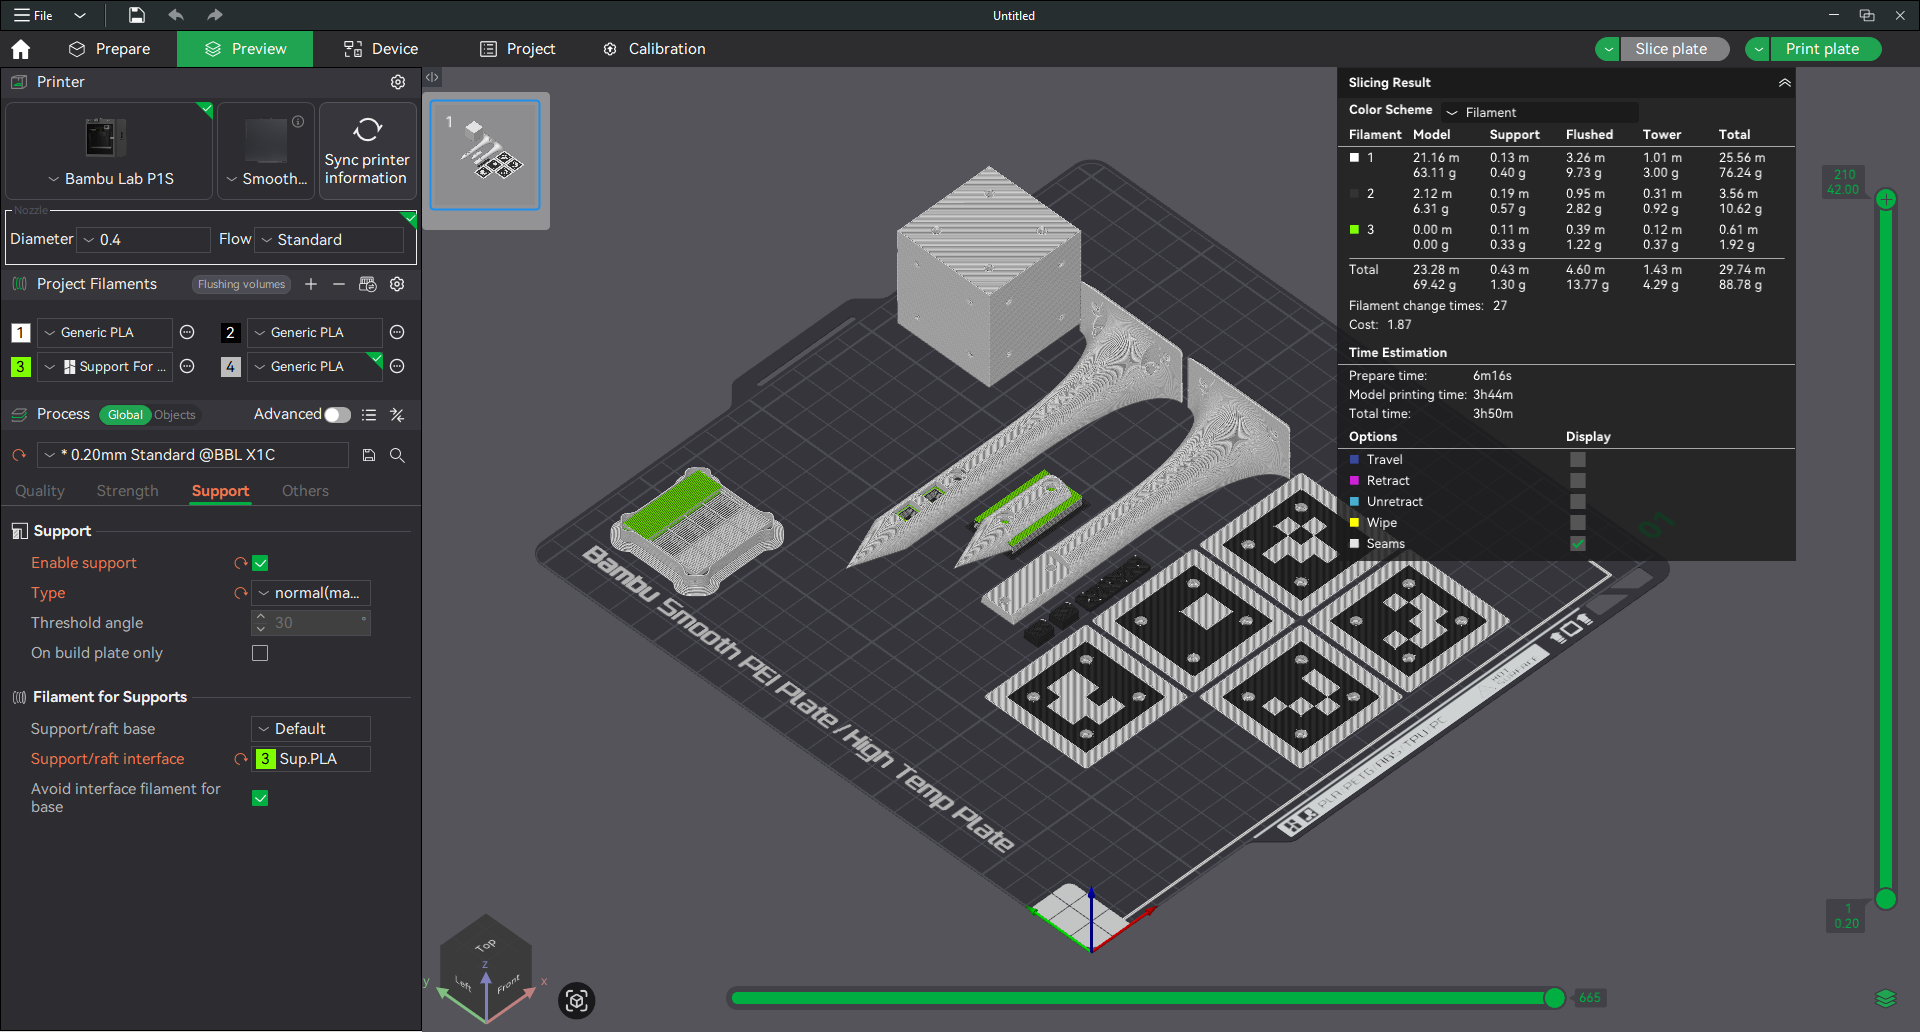
\includegraphics[width=0.95\linewidth]{img/appendix/pen_slice_side.png}
    \caption{3D printing plate layout (slicer screenshot).}
    \label{fig:app_print_layout}
\end{figure}

\subsection{Scene registry example}
\label{appendix:scene_registry}

The scene detection pipeline relies on a JSON registry describing fiducial-tagged box objects (marker ID, marker size, box dimensions, and the marker-to-object transform).
An example registry instance used in this thesis is:

\begin{verbatim}
[
  {
    "markerId": 60,
    "marker_size": 0.036,
    "size_x": 0.048,
    "size_y": 0.048,
    "size_z": 0.048,
    "T_marker_pose_": {
      "position": {"x": 0.0, "y": 0.0, "z": -0.024},
      "orientation": {"qx": 0.0, "qy": 0.0, "qz": 0.0, "qw": 1.0}
    }
  }
]
\end{verbatim}

In the submitted source tree, the example registry file is located at
\path{diploma-thesis-code/default_modules/scene_detection_stereocam_module/module_data/registered_objects.json}.
After installation, it is copied to the runtime data directory as
\path{binaries/data/scene_detection_stereocam_module/registered_objects.json}.

\subsection{Example scene CAD model}
\label{appendix:scene_cad}

A simple example box model used for visualization and documentation is provided as:
\path{scene/scene_box.step}. The 3D printing settings for this model were the same as the pen, just without supports. 
Render of this example box is shown in \autoref{fig:app_scene_box}.

\begin{figure}[h]
    \centering
    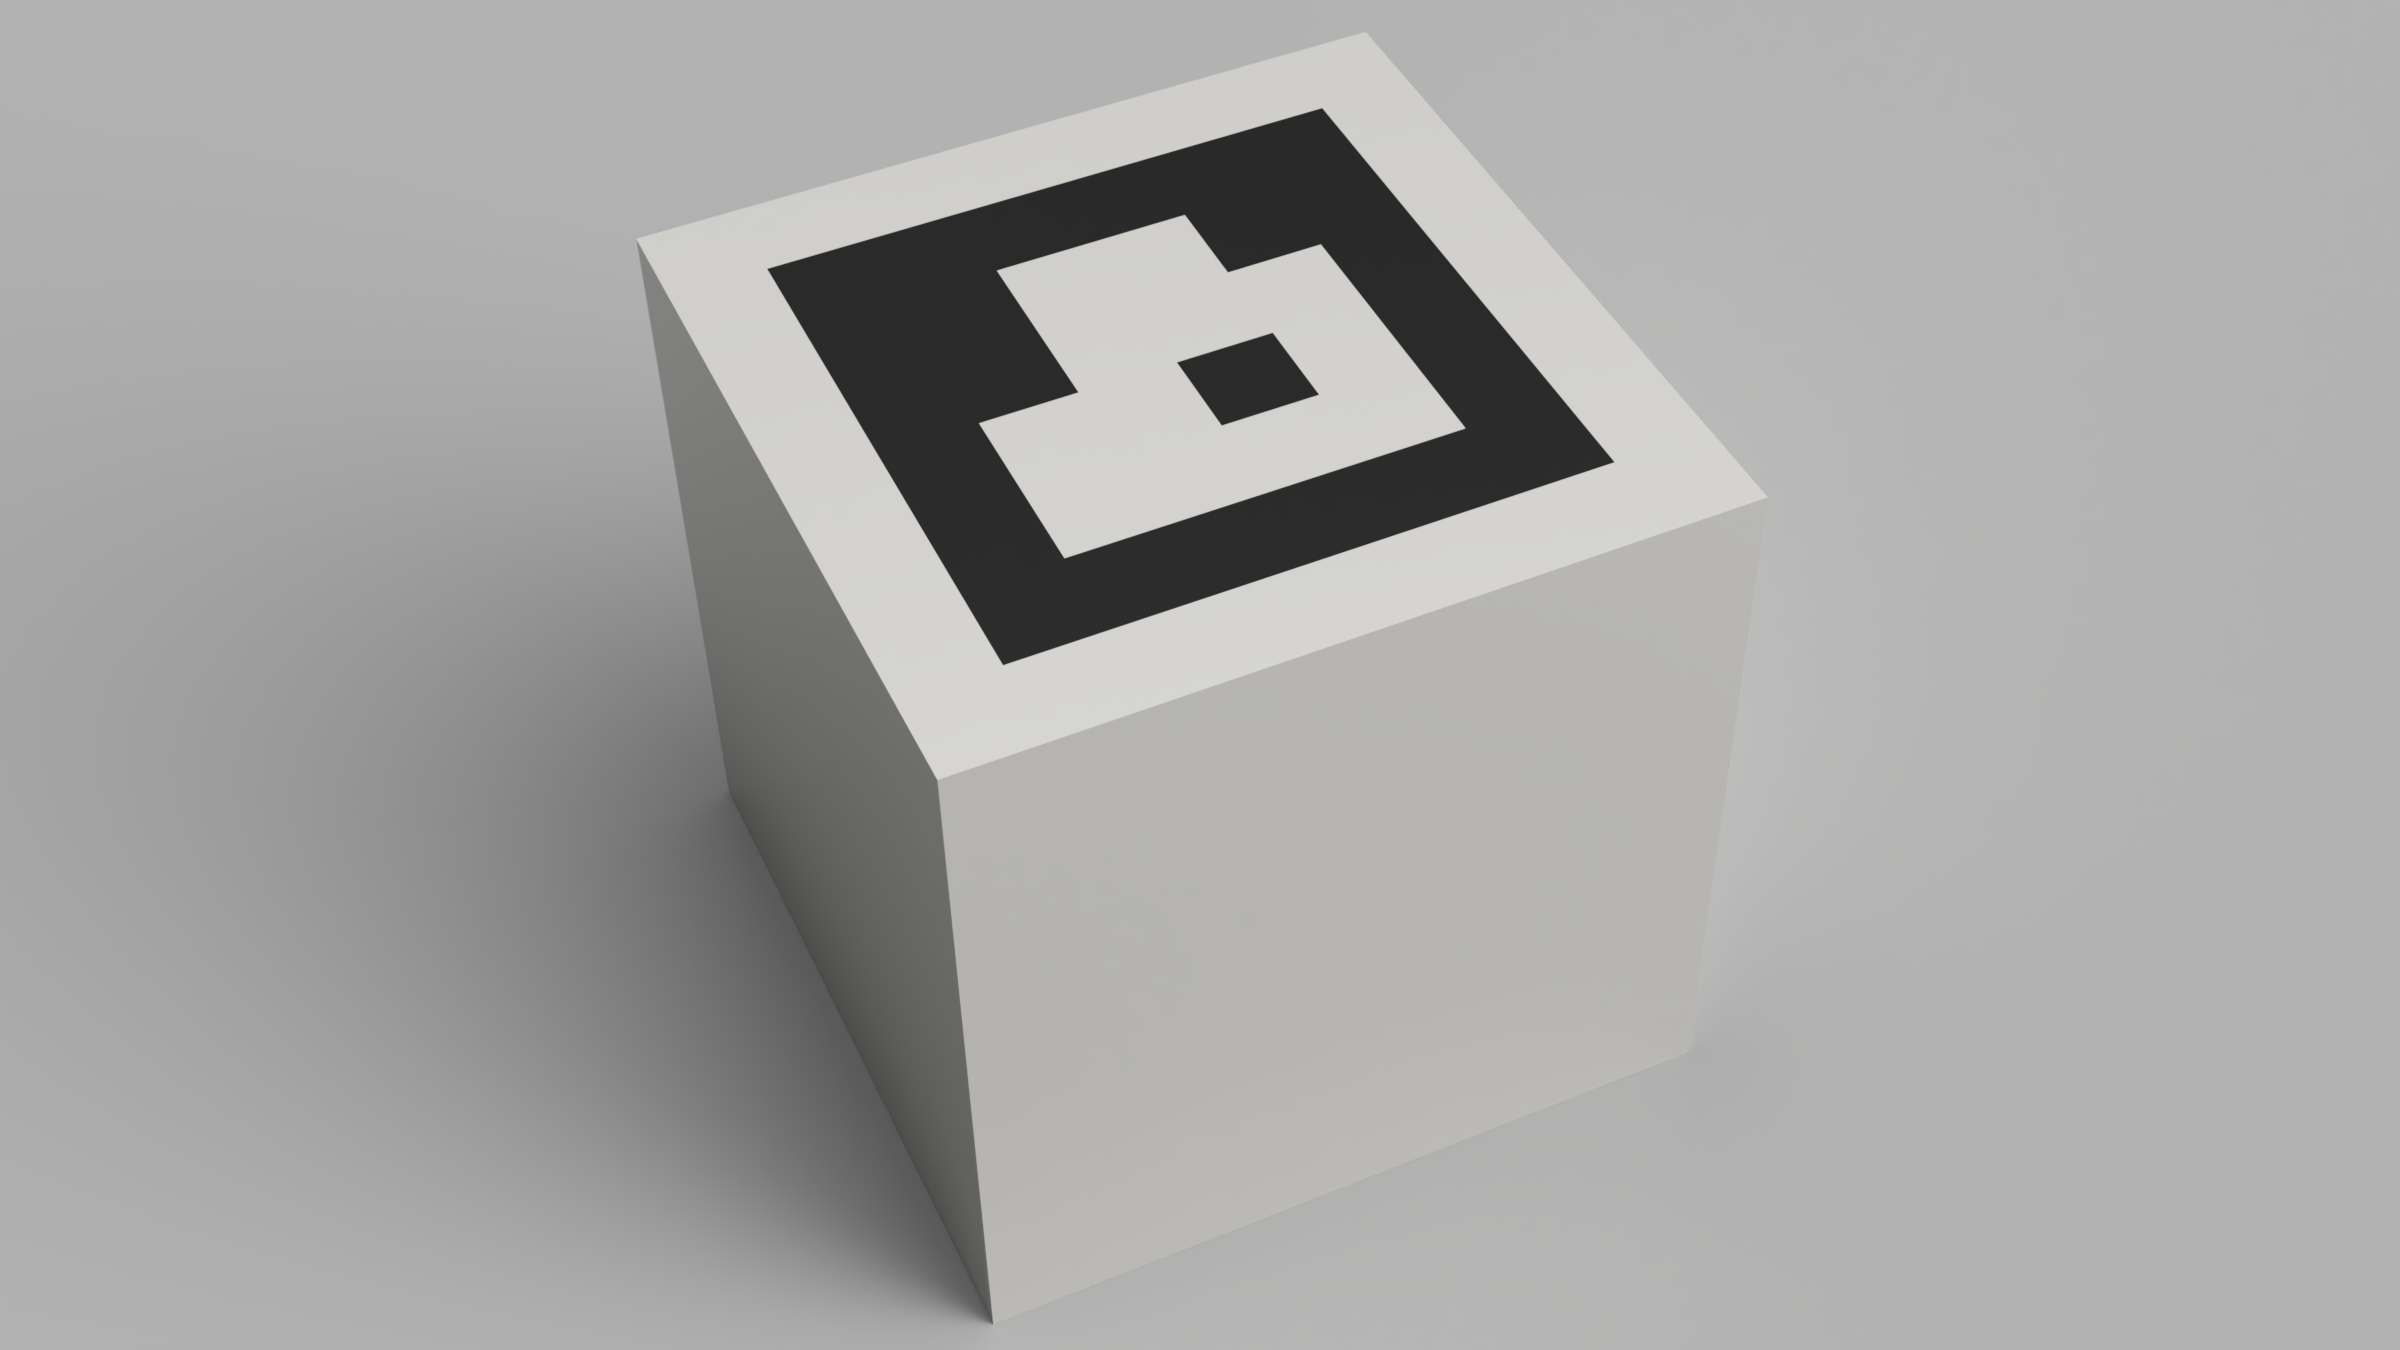
\includegraphics[width=0.6\linewidth]{img/appendix/scene_box_bg.png}
    \caption{Example fiducial-tagged box scene object (CAD render).}
    \label{fig:app_scene_box}
\end{figure}

\subsection{Robot-side component (CBun) and reproducibility boundary}
\label{appendix:cbun}

The prototype uses a robot-side component (CBun) that runs on the Kassow controller and exposes the robot capabilities over a network endpoint.
On the thesis side, \type{robot\_module\_kassow} consumes this endpoint and implements the \type{robot\_interface} protocol towards the rest of the runtime.

The CBun source tree is included in the attachment under:
\path{robot/aergo_interface_cbun/}.
It is not part of the runtime module graph shown in \autoref{fig:runtime_full}; it is deployed to the robot controller separately and communicates with the \type{robot\_module\_kassow} module.

\minihead{Build overview.}
The CBun build depends on Kassow-provided development libraries and is therefore built inside a preconfigured development container.
A practical build workflow used during development is:

\begin{itemize}
    \item Install Docker (required by VS Code Dev Containers).
    \item The workflow was verified with VS Code 1.85.2. Newer VS Code releases may fail to attach to the provided devcontainer due to compatibility constraints of the container image.
    \item Open \path{robot/aergo_interface_cbun/} in VS Code.
    \item Use the ``Dev Containers'' extension and ``Reopen in Container''.
    \item Configure CMake with \path{backend/CMakeLists.txt} and toolchain ``GCC 8.4.0''.
    \item Build the target using the provided build task (e.g., ``CBun: Clean Build'').
\end{itemize}

The resulting CBun bundle is produced at:
\path{robot/aergo_interface_cbun/build/aergo_adapter.cbun}.
Deployment then consists of copying this bundle to removable media and installing it on the robot controller.
\xxx{Keep detailed robot-side installation steps in Chapter~\ref{chapter:ch5_user_workflow} (operator procedure), and keep this appendix limited to build and artifact location.  --> keep this xxx here, so i dont forget.}

\minihead{Reproducibility limitation.}
Executing the full end-to-end system requires either access to a physical Kassow robot or a compatible offline environment (e.g., REMII).
At the time of development, access to REMII is restricted to Kassow partners/users.